\documentclass[12pt,a4paper]{article}

\usepackage[utf8]{inputenc}
\usepackage{babel}
\babelprovide[main,import]{portuguese}
\usepackage{geometry}
\usepackage{graphicx}
\usepackage{booktabs}
\usepackage{amsmath}
\usepackage{array}
\usepackage[protrusion=true,expansion=false]{microtype}
\usepackage{hyperref}

\geometry{margin=2.5cm}
\graphicspath{{../images/}}
\setlength{\emergencystretch}{2em}

\title{Predi\c{c}\~ao da Qualidade de Vinhos por Atributos F\'isico-Qu\'imicos com Modelos de Aprendizagem de M\'aquina Implementados Manualmente}
\author{Gabriel de Sousa Cavalcante \and Gabriel Matias de Almeida \and Maria Elaine de Holanda Cavalcante \and Edileudo Maciel Moreira Filho}
\date{2026}

\begin{document}

\maketitle

\begin{abstract}
Este artigo avalia modelos de aprendizagem de m\'aquina para predizer a qualidade sensorial de vinhos a partir de propriedades f\'isico-qu\'imicas. Foram utilizados os arquivos de vinho tinto e vinho branco da base \textit{Wine Quality}, associados ao Vinho Verde portugu\^es, totalizando 6.497 amostras, 11 atributos laboratoriais originais e uma vari\'avel indicadora do tipo de vinho. O problema foi formulado de duas maneiras: regress\~ao da nota original de qualidade e classifica\c{c}\~ao ordinal em tr\^es faixas, definidas por notas baixas ($y \leq 5$), intermedi\'arias ($y=6$) e altas ($y \geq 7$). O protocolo experimental utilizou separa\c{c}\~ao treino--teste estratificada por nota original e tipo de vinho, padroniza\c{c}\~ao ajustada apenas no treino de cada etapa, baselines triviais, valida\c{c}\~ao cruzada manual para hiperpar\^ametros selecionados e avalia\c{c}\~ao repetida em cinco divis\~oes. Os modelos avaliados foram Random Forest para regress\~ao, K-Nearest Neighbors para regress\~ao e classifica\c{c}\~ao, e Regress\~ao Softmax para classifica\c{c}\~ao multiclasse, todos implementados sem estimadores prontos de bibliotecas especializadas. No particionamento principal, a Random Forest obteve o melhor desempenho geral, com RMSE de 0,6235 na regress\~ao, contra 0,8746 do baseline pela m\'edia do treino, e AUC-ROC macro de 0,8582 ap\'os convers\~ao das predi\c{c}\~oes para classes. Em cinco divis\~oes repetidas, o mesmo modelo apresentou RMSE m\'edio de 0,6225 com IC95 de 0,0023. Apesar disso, a revoca\c{c}\~ao para vinhos de alta qualidade permaneceu limitada, evidenciando o impacto do desbalanceamento e da proximidade entre classes adjacentes.
\end{abstract}

\noindent\textbf{Palavras-chave:} aprendizagem de m\'aquina; qualidade de vinhos; Random Forest; KNN; regress\~ao softmax; classifica\c{c}\~ao ordinal.

\section{Introdu\c{c}\~ao}
\label{sec:introducao}

A avalia\c{c}\~ao da qualidade de vinhos combina medi\c{c}\~oes objetivas, experi\^encia enol\'ogica e julgamento sensorial. Atributos como acidez, teor alco\'olico, densidade, pH, concentra\c{c}\~ao de a\c{c}\'ucar residual e compostos de enxofre podem ser medidos em laborat\'orio, mas a nota final de qualidade resulta de avalia\c{c}\~oes humanas e, portanto, cont\'em componentes subjetivos. Essa combina\c{c}\~ao torna a base \textit{Wine Quality} um caso relevante para investigar at\'e que ponto vari\'aveis f\'isico-qu\'imicas explicam prefer\^encias sensoriais.

O conjunto de dados, disponibilizado no UCI Machine Learning Repository, foi introduzido por Cortez et al.~\cite{cortez2009modeling,uciWineQuality}. Ele cont\'em amostras de vinhos tintos e brancos da regi\~ao portuguesa do Vinho Verde, com 11 vari\'aveis de entrada obtidas por testes laboratoriais e uma vari\'avel de sa\'ida, \texttt{quality}, registrada como nota inteira entre 0 e 10. Segundo a descri\c{c}\~ao da base, a nota corresponde \`a mediana de pelo menos tr\^es avalia\c{c}\~oes feitas por especialistas. A base pode ser estudada tanto como regress\~ao quanto como classifica\c{c}\~ao, e suas classes s\~ao ordenadas e desbalanceadas.

A pergunta central deste trabalho \'e: \textit{qual formula\c{c}\~ao e qual fam\'ilia de modelos, entre as implementadas manualmente, apresentam melhor desempenho para estimar a qualidade do vinho a partir dos atributos f\'isico-qu\'imicos dispon\'iveis?} Para responder a essa pergunta, foram comparados modelos com diferentes vieses indutivos: uma Random Forest manual para regress\~ao, um K-Nearest Neighbors (KNN) manual para regress\~ao e classifica\c{c}\~ao, e uma Regress\~ao Softmax manual para classifica\c{c}\~ao multiclasse.

O estudo tem tr\^es contribui\c{c}\~oes principais. Primeiro, apresenta um protocolo experimental reprodut\'ivel, com separa\c{c}\~ao estratificada, preven\c{c}\~ao expl\'icita de vazamento de informa\c{c}\~ao e m\'etricas apropriadas ao desbalanceamento. Segundo, compara diretamente a regress\~ao da nota original com a classifica\c{c}\~ao em tr\^es faixas de qualidade, preservando a interpreta\c{c}\~ao ordinal do alvo. Terceiro, documenta implementa\c{c}\~oes manuais dos algoritmos, das m\'etricas e da valida\c{c}\~ao cruzada, deixando expl\'icitas decis\~oes que normalmente ficam encapsuladas em bibliotecas.

O artigo est\'a organizado da seguinte forma. A Se\c{c}\~ao~\ref{sec:fundamentacao} apresenta a base de dados, as formula\c{c}\~oes do problema e os modelos avaliados. A Se\c{c}\~ao~\ref{sec:metodologia} descreve o protocolo experimental. A Se\c{c}\~ao~\ref{sec:resultados} apresenta e discute os resultados. A Se\c{c}\~ao~\ref{sec:limitacoes} explicita limita\c{c}\~oes e amea\c{c}as \`a validade. Por fim, a Se\c{c}\~ao~\ref{sec:conclusao} resume as conclus\~oes.

\section{Fundamenta\c{c}\~ao e Dados}
\label{sec:fundamentacao}

\subsection{Base \textit{Wine Quality}}
\label{subsec:dataset}

A base \textit{Wine Quality} cont\'em dois arquivos: 1.599 amostras de vinho tinto e 4.898 amostras de vinho branco. Embora Cortez et al.~\cite{cortez2009modeling} apresentem os dois subconjuntos separadamente, neste trabalho eles foram concatenados para aumentar o n\'umero de exemplos dispon\'iveis e avaliar um modelo \'unico para a base combinada. Para preservar informa\c{c}\~ao sobre o tipo de vinho, foi acrescentada a vari\'avel bin\'aria \texttt{is\_red}, igual a 1 para vinhos tintos e 0 para vinhos brancos. Assim, o conjunto final possui 6.497 inst\^ancias e 12 atributos de entrada. As 11 vari\'aveis f\'isico-qu\'imicas originais s\~ao: acidez fixa, acidez vol\'atil, \'acido c\'itrico, a\c{c}\'ucar residual, cloretos, di\'oxido de enxofre livre, di\'oxido de enxofre total, densidade, pH, sulfatos e teor alco\'olico.

A vari\'avel alvo, \texttt{quality}, \'e uma nota sensorial discreta. Embora a escala nominal v\'a de 0 a 10, no conjunto utilizado as notas observadas variam de 3 a 9. A distribui\c{c}\~ao \'e concentrada em notas intermedi\'arias, especialmente 5 e 6, com poucos exemplos nos extremos. Esse padr\~ao afeta a avalia\c{c}\~ao de classificadores, pois m\'etricas agregadas, como acur\'acia, podem favorecer as categorias mais frequentes.

Outra caracter\'istica importante \'e a exist\^encia de correla\c{c}\~oes entre atributos. O di\'oxido de enxofre total inclui a fra\c{c}\~ao livre, o que explica a correla\c{c}\~ao positiva esperada entre essas vari\'aveis. Tamb\'em s\~ao esperadas rela\c{c}\~oes qu\'imicas entre densidade, teor alco\'olico e a\c{c}\'ucar residual: em geral, maior teor alco\'olico reduz a densidade, enquanto maior a\c{c}\'ucar residual tende a aument\'a-la. Esses padr\~oes sugerem que modelos capazes de capturar intera\c{c}\~oes n\~ao lineares podem ser vantajosos.

\subsection{Formula\c{c}\~oes do problema}
\label{subsec:formulacoes}

Foram adotadas duas formula\c{c}\~oes supervisionadas. Na regress\~ao, o objetivo \'e estimar diretamente a nota $y$ a partir do vetor de atributos $\mathbf{x}$, produzindo uma predi\c{c}\~ao real $\hat{y}$. Essa abordagem preserva a escala original e permite medir erro num\'erico.

Na classifica\c{c}\~ao, a nota foi agrupada em tr\^es classes ordinais:

\begin{equation}
c(y) =
\begin{cases}
0, & y \leq 5{,}5,\\
1, & 5{,}5 < y < 6{,}5,\\
2, & y \geq 6{,}5.
\end{cases}
\label{eq:classes}
\end{equation}

Para notas inteiras, a Equa\c{c}\~ao~\ref{eq:classes} equivale \`as regras $y \leq 5$ para a classe ruim, $y=6$ para a classe mediana e $y \geq 7$ para a classe boa. A mesma fun\c{c}\~ao foi aplicada \`as sa\'idas cont\'inuas dos regressores, o que permite comparar diretamente regressores convertidos em classificadores e classificadores treinados diretamente sobre as classes.

Embora as classes possuam uma ordem natural, os classificadores usados neste trabalho foram treinados como modelos multiclasse convencionais. Portanto, eles n\~ao incorporam explicitamente uma fun\c{c}\~ao de perda ordinal que penalize diferentemente erros adjacentes e erros extremos.

\subsection{Modelos avaliados}
\label{subsec:modelos}

A Random Forest combina v\'arias \'arvores de decis\~ao constru\'idas com aleatoriedade na amostragem das observa\c{c}\~oes e na sele\c{c}\~ao de atributos candidatos em cada divis\~ao \cite{breiman2001random}. Neste trabalho, foi implementada uma Random Forest de regress\~ao baseada em \'arvores CART \cite{breiman1984cart}. Cada \'arvore foi ajustada sobre uma amostra bootstrap do treino, e a predi\c{c}\~ao final foi a m\'edia das predi\c{c}\~oes das \'arvores. As divis\~oes foram escolhidas por redu\c{c}\~ao da soma dos erros quadr\'aticos.

O K-Nearest Neighbors \'e um m\'etodo n\~ao param\'etrico baseado em inst\^ancias \cite{cover1967nearest}. Para cada amostra de teste, o algoritmo identifica os $k$ exemplos de treino mais pr\'oximos segundo dist\^ancia euclidiana no espa\c{c}o padronizado. Na regress\~ao, a predi\c{c}\~ao \'e a m\'edia das notas dos vizinhos. Na classifica\c{c}\~ao, as probabilidades de classe s\~ao estimadas pela frequ\^encia relativa das classes entre os vizinhos.

A Regress\~ao Softmax, ou regress\~ao log\'istica multinomial, modela probabilidades de classe a partir de fun\c{c}\~oes lineares dos atributos \cite{bishop2006pattern}. Para uma amostra $\mathbf{x}$ e classe $k$, o modelo calcula

\begin{equation}
P(y=k \mid \mathbf{x}) =
\frac{\exp(\mathbf{w}_k^{T}\mathbf{x})}
{\sum_{\ell=1}^{K}\exp(\mathbf{w}_{\ell}^{T}\mathbf{x})}.
\label{eq:softmax}
\end{equation}

Os pesos foram ajustados por descida do gradiente, minimizando entropia cruzada multiclasse com regulariza\c{c}\~ao L2. Para reduzir o efeito do desbalanceamento, cada amostra recebeu peso inversamente proporcional \`a frequ\^encia de sua classe no conjunto de treino. Esse tratamento foi aplicado apenas ao classificador Softmax, pois os regressores foram treinados diretamente sobre a nota cont\'inua e s\'o depois convertidos para classes; portanto, a compara\c{c}\~ao entre formula\c{c}\~oes n\~ao elimina completamente a assimetria causada pelo desbalanceamento.

\section{Metodologia}
\label{sec:metodologia}

\subsection{Protocolo experimental}
\label{subsec:protocolo}

O pipeline foi implementado no arquivo \texttt{wine\_quality.py}. A execu\c{c}\~ao principal utilizou semente fixa igual a 42; al\'em dela, a avalia\c{c}\~ao final foi repetida com cinco sementes para estimar a variabilidade por particionamento. O procedimento executado foi:

\begin{enumerate}
    \item carregar os arquivos \texttt{winequality-red.csv} e \texttt{winequality-white.csv};
    \item adicionar a vari\'avel \texttt{is\_red} e concatenar as amostras;
    \item verificar explicitamente a aus\^encia de valores faltantes e relatar linhas duplicadas antes da divis\~ao;
    \item construir os alvos de regress\~ao e classifica\c{c}\~ao;
    \item separar treino e teste em propor\c{c}\~ao 80/20, com estratifica\c{c}\~ao pelo cruzamento entre \texttt{quality} original e \texttt{is\_red};
    \item padronizar os atributos usando m\'edia e desvio padr\~ao estimados apenas no treino;
    \item calcular baselines triviais usando apenas o conjunto de treino;
    \item selecionar hiperpar\^ametros por valida\c{c}\~ao cruzada manual quando aplic\'avel;
    \item treinar os modelos finais no treino completo, avaliar no teste reservado e repetir a avalia\c{c}\~ao em m\'ultiplas divis\~oes com os hiperpar\^ametros selecionados.
\end{enumerate}

A padroniza\c{c}\~ao foi aplicada a todos os atributos. Para cada atributo $j$, com m\'edia $\mu_j$ e desvio padr\~ao $\sigma_j$ calculados no treino, a transforma\c{c}\~ao usada foi

\begin{equation}
x'_{ij} = \frac{x_{ij} - \mu_j}{\sigma_j}.
\label{eq:standardization}
\end{equation}

Esse cuidado \'e essencial para o KNN, pois dist\^ancias euclidianas s\~ao sens\'iveis \`a escala dos atributos, e tamb\'em melhora a estabilidade num\'erica da Regress\~ao Softmax. Durante a valida\c{c}\~ao cruzada, a m\'edia e o desvio padr\~ao foram recalculados dentro de cada dobra usando apenas o subtreino da dobra, e depois aplicados \`a valida\c{c}\~ao correspondente.

\subsection{Hiperpar\^ametros}
\label{subsec:hiperparametros}

A sele\c{c}\~ao de hiperpar\^ametros foi feita exclusivamente no conjunto de treino. As dobras foram estratificadas pelo cruzamento entre nota original e tipo de vinho. Para regress\~ao com KNN, foram usadas cinco dobras e o crit\'erio foi o menor RMSE m\'edio. Para classifica\c{c}\~ao com KNN e Regress\~ao Softmax, foram usadas cinco dobras e o crit\'erio foi a maior AUC-ROC macro no esquema um-contra-resto.

No KNN, foram testados $k \in \{3,5,7,9,11\}$ para regress\~ao e classifica\c{c}\~ao. Na Regress\~ao Softmax, a for\c{c}a da regulariza\c{c}\~ao L2 foi selecionada em uma grade logar\'itmica entre $10^{-4}$ e $1$. Na Random Forest, foi usada uma busca pequena em tr\^es dobras com 60 \'arvores por configura\c{c}\~ao, variando profundidade m\'axima, m\'inimo de amostras para divis\~ao, m\'inimo de amostras por folha e n\'umero de atributos considerados por n\'o. O modelo final de Random Forest foi treinado com 120 \'arvores, amostragem bootstrap e 32 candidatos a ponto de corte por atributo avaliado.

\subsection{M\'etricas}
\label{subsec:metricas}

Para regress\~ao, foram usados RMSE, MAE e $R^2$:

\begin{equation}
\mathrm{RMSE} = \sqrt{\frac{1}{n}\sum_{i=1}^{n}(y_i-\hat{y}_i)^2},
\quad
\mathrm{MAE} = \frac{1}{n}\sum_{i=1}^{n}|y_i-\hat{y}_i|.
\end{equation}

O coeficiente $R^2$ foi calculado como a propor\c{c}\~ao da variabilidade do alvo explicada pelo modelo em rela\c{c}\~ao a uma predi\c{c}\~ao constante pela m\'edia.

Para classifica\c{c}\~ao, foram calculadas acur\'acia, F1 macro, precis\~ao e revoca\c{c}\~ao por classe, matrizes de confus\~ao e AUC-ROC macro um-contra-resto. A AUC-ROC \'e especialmente \'util para comparar modelos por capacidade de ranqueamento em diferentes limiares \cite{fawcett2006roc}; sua generaliza\c{c}\~ao multiclasse foi usada por m\'edia macro das AUCs um-contra-resto \cite{hand2001auc}. Para os regressores convertidos em classes, os escores de ranqueamento foram definidos como $s_0=-\hat{y}$ para a classe ruim, $s_1=-|\hat{y}-6|$ para a classe mediana e $s_2=\hat{y}$ para a classe boa.

Dois baselines foram inclu\'idos para calibrar a interpreta\c{c}\~ao dos resultados. Na regress\~ao, o baseline prediz sempre a m\'edia da nota observada no treino. Na classifica\c{c}\~ao, o baseline prediz sempre a classe majorit\'aria do treino, que corresponde \`a classe mediana. Para uma verifica\c{c}\~ao simples de sobreajuste, tamb\'em foram calculadas m\'etricas no pr\'oprio conjunto de treino, usando os modelos finais ajustados no treino completo. Para estimar a sensibilidade ao particionamento, os modelos finais foram reavaliados em cinco divis\~oes estratificadas com sementes distintas, mantendo fixos os hiperpar\^ametros selecionados na execu\c{c}\~ao principal; os intervalos de confian\c{c}a foram calculados como $1{,}96$ vezes o erro padr\~ao das cinco estimativas.

\section{Experimentos e Resultados}
\label{sec:resultados}

\subsection{Particionamento e distribui\c{c}\~ao das classes}
\label{subsec:distribuicao}

O conjunto final possui 6.497 amostras e 12 atributos de entrada. N\~ao foram encontrados valores ausentes. Antes da divis\~ao treino--teste, foram identificadas 1.177 linhas repetidas, correspondentes a 992 padr\~oes duplicados; elas foram relatadas, mas mantidas para preservar a base original. A separa\c{c}\~ao estratificada por nota original e tipo de vinho produziu 5.196 amostras de treino e 1.301 amostras de teste. A Tabela~\ref{tab:distribuicao-classes} mostra que as propor\c{c}\~oes das classes foram preservadas.

\begin{table}[htbp]
\centering
\caption{Distribui\c{c}\~ao das classes no conjunto completo, treino e teste.}
\label{tab:distribuicao-classes}
\begin{tabular}{lrrrr}
\toprule
Classe & Regra & Total & Treino & Teste \\
\midrule
Ruim & $y \leq 5$ & 2384 & 1907 & 477 \\
Mediano & $y = 6$ & 2836 & 2268 & 568 \\
Bom & $y \geq 7$ & 1277 & 1021 & 256 \\
\bottomrule
\end{tabular}
\end{table}

\begin{figure}[htbp]
\centering
\begin{minipage}{0.48\textwidth}
\centering
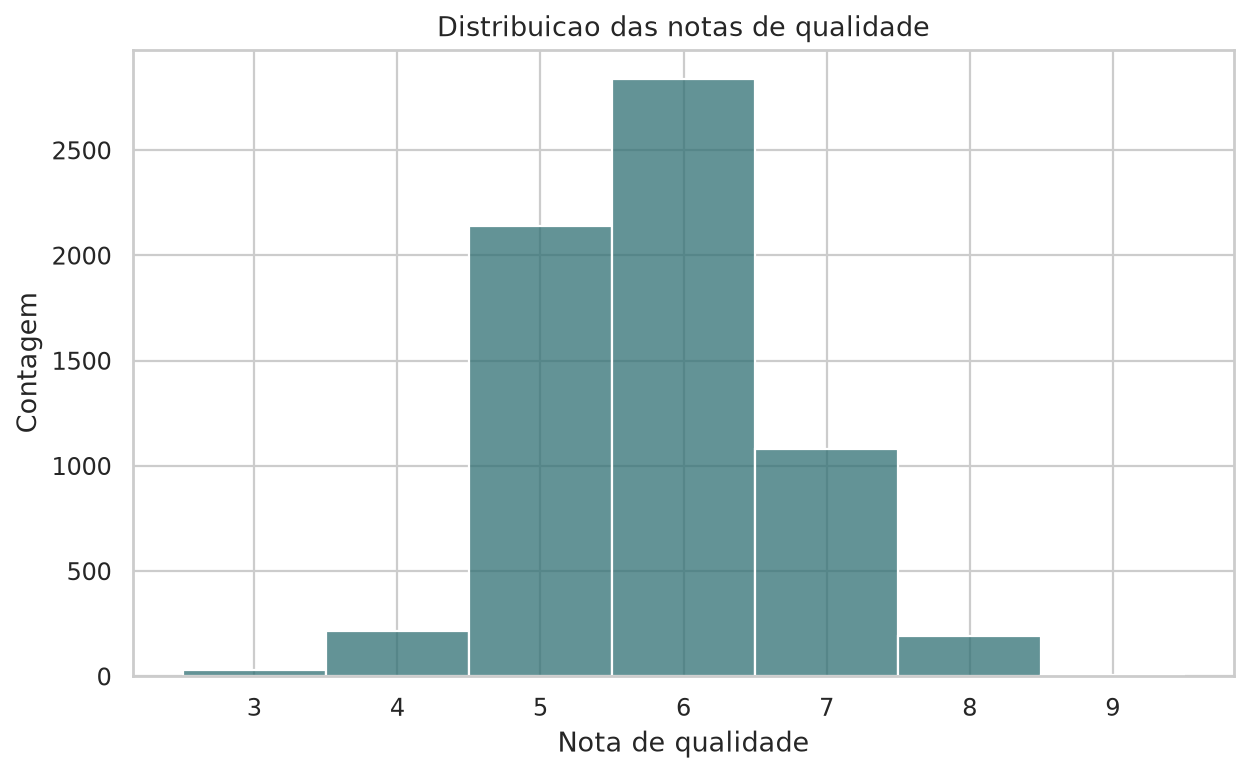
\includegraphics[width=\linewidth]{quality_distribution.png}
\end{minipage}
\hfill
\begin{minipage}{0.48\textwidth}
\centering
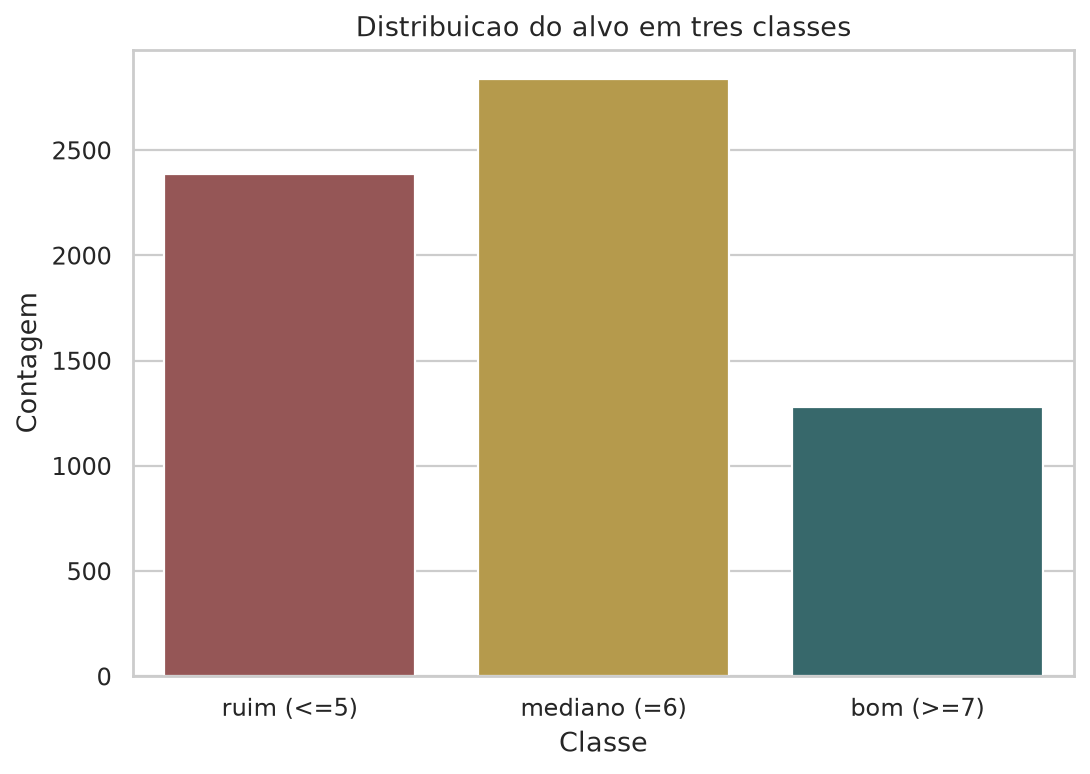
\includegraphics[width=\linewidth]{class_distribution_three_classes.png}
\end{minipage}
\caption{Distribui\c{c}\~ao das notas originais e das tr\^es classes de qualidade.}
\label{fig:eda-distribuicoes}
\end{figure}

A Figura~\ref{fig:eda-distribuicoes} confirma a concentra\c{c}\~ao em notas intermedi\'arias. A classe boa representa apenas 19,7\% do total, o que justifica o uso de F1 macro, AUC-ROC macro e m\'etricas por classe al\'em da acur\'acia.

\subsection{An\'alise explorat\'oria}
\label{subsec:analise-exploratoria}

A matriz de correla\c{c}\~ao de Pearson apresentada na Figura~\ref{fig:correlacao} evidencia padr\~oes coerentes com a estrutura qu\'imica dos dados. A correla\c{c}\~ao entre di\'oxido de enxofre livre e total foi 0,721. A densidade apresentou correla\c{c}\~ao negativa com \'alcool (-0,687) e positiva com a\c{c}\'ucar residual (0,553). Em rela\c{c}\~ao \`a nota de qualidade, o teor alco\'olico teve correla\c{c}\~ao positiva moderada (0,444), enquanto a acidez vol\'atil teve correla\c{c}\~ao negativa (-0,266). Esses valores sugerem associa\c{c}\~oes individuais relevantes, mas n\~ao s\~ao suficientes para explicar a qualidade sem modelos multivariados.

\begin{figure}[htbp]
\centering
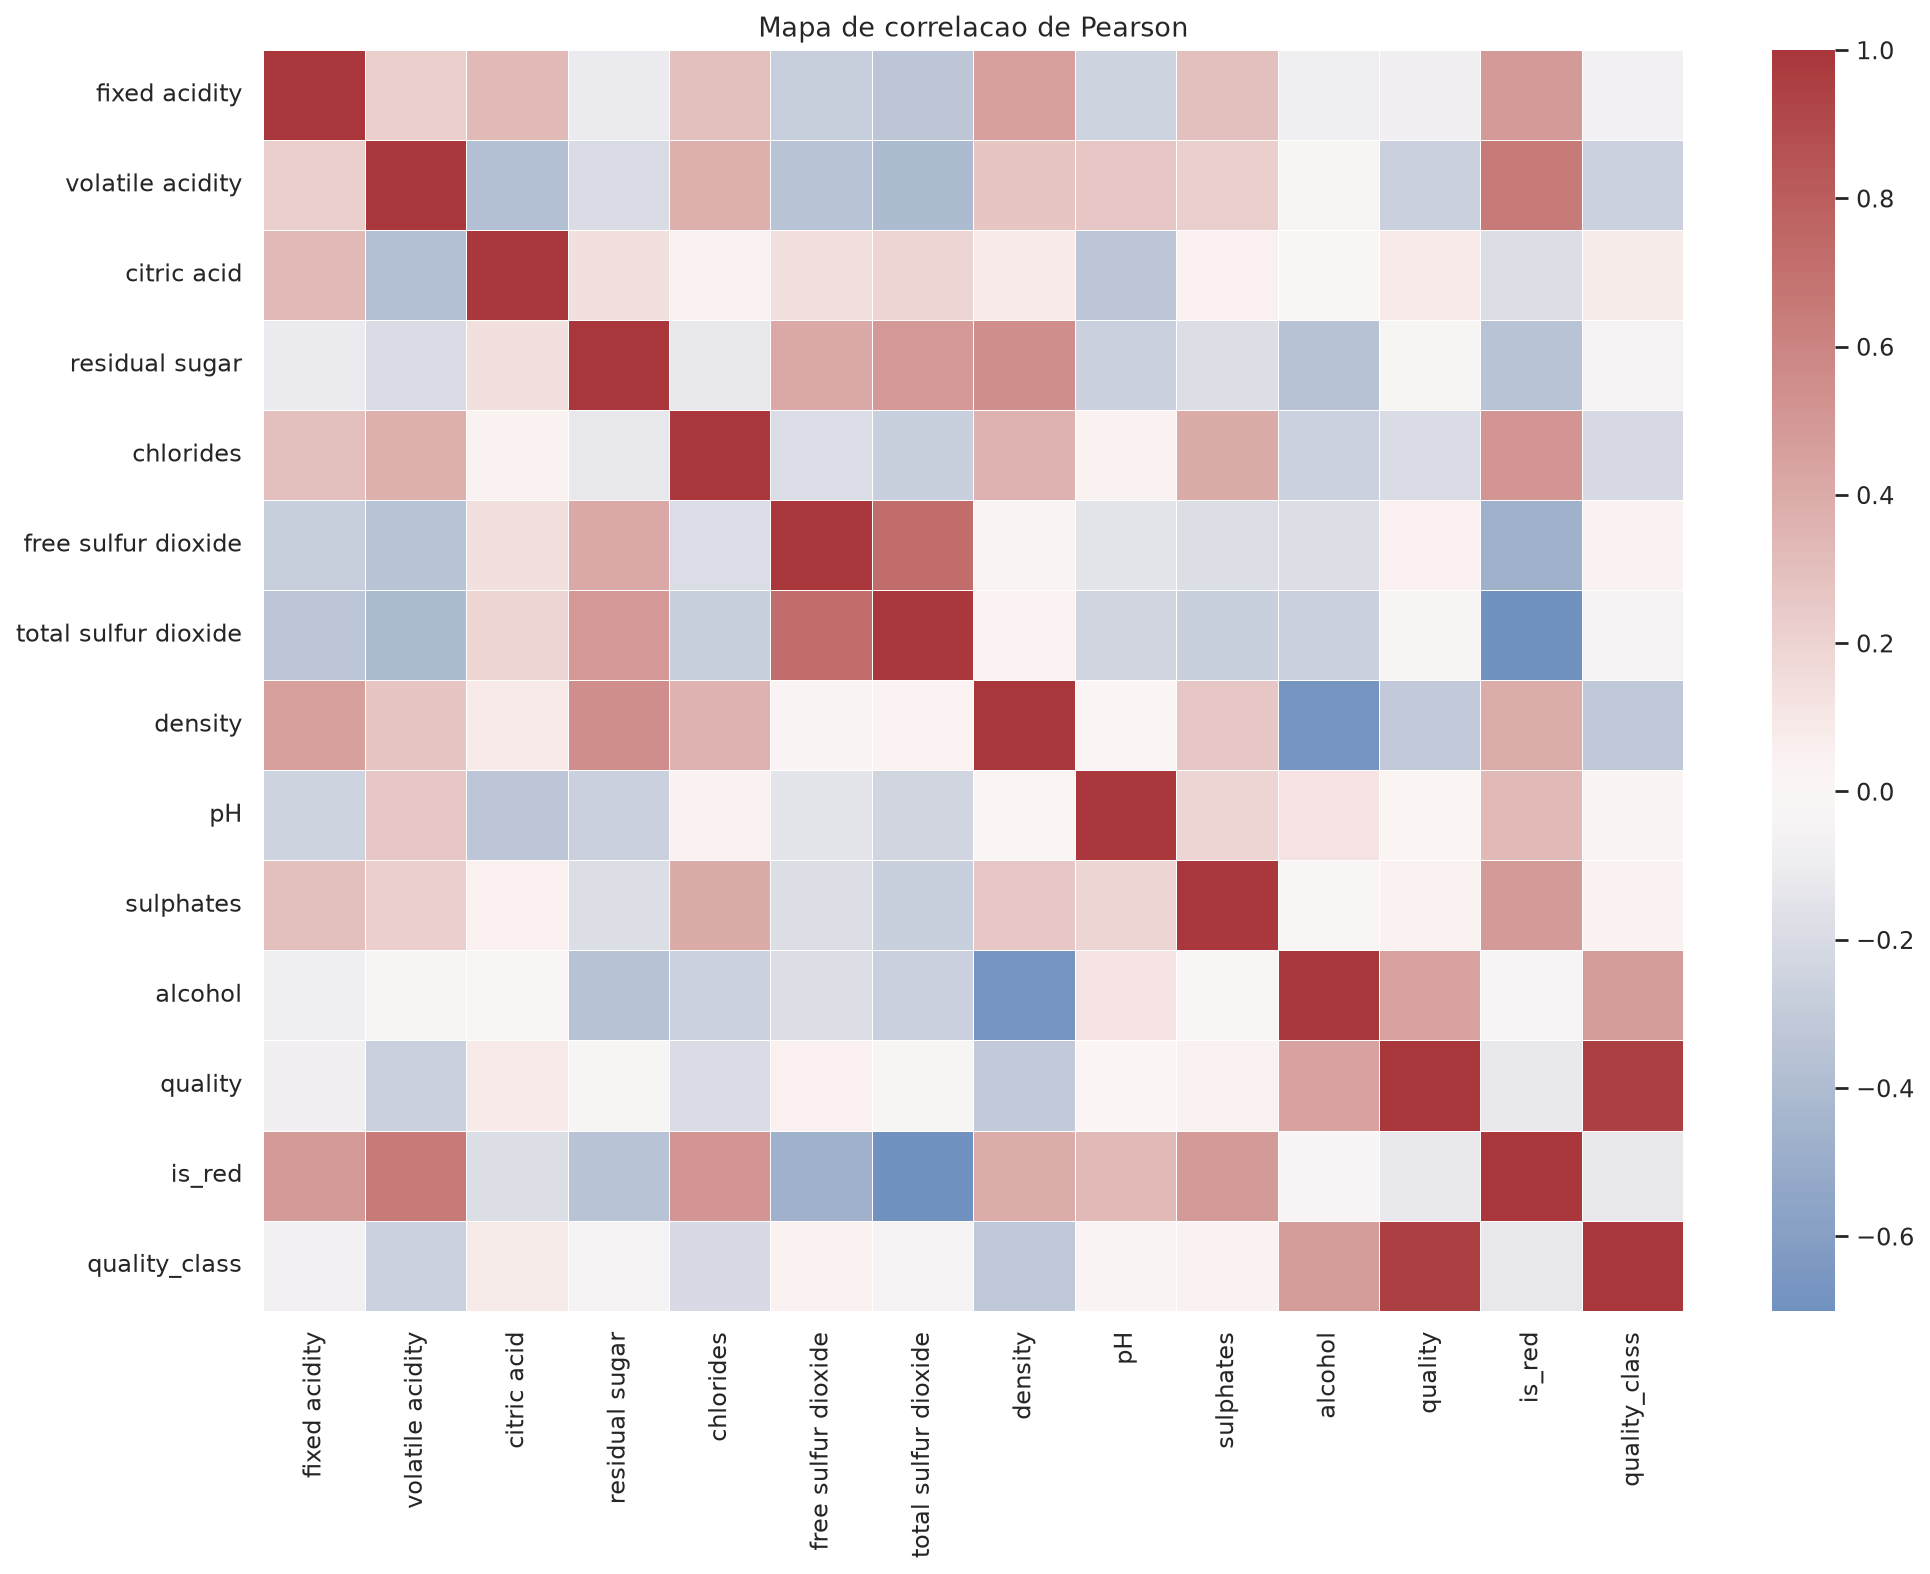
\includegraphics[width=0.90\textwidth]{correlation_heatmap.png}
\caption{Mapa de correla\c{c}\~ao de Pearson entre atributos, nota e classe de qualidade.}
\label{fig:correlacao}
\end{figure}

\subsection{Valida\c{c}\~ao cruzada}
\label{subsec:validacao}

A Tabela~\ref{tab:validacao-cruzada} resume os hiperpar\^ametros selecionados por valida\c{c}\~ao cruzada. O valor $k=11$ foi selecionado para o KNN Regressor e $k=7$ para o KNN Classifier. Na Regress\~ao Softmax, a melhor regulariza\c{c}\~ao foi $\lambda=0{,}000316$. Na Random Forest, a busca favoreceu \'arvores mais profundas, com profundidade m\'axima 18.

\begin{table}[htbp]
\centering
\caption{Hiperpar\^ametros selecionados por valida\c{c}\~ao cruzada.}
\label{tab:validacao-cruzada}
\resizebox{\textwidth}{!}{%
\begin{tabular}{lllr}
\toprule
Modelo & Hiperpar\^ametro & Crit\'erio & Valor de valida\c{c}\~ao \\
\midrule
Random Forest Regressor & prof. 18; split 8; folha 3; $\sqrt{p}$ & menor RMSE & 0,6456 \\
KNN Regressor & $k=11$ & menor RMSE & 0,7083 \\
KNN Classifier & $k=7$ & maior AUC-ROC macro & 0,7671 \\
Softmax Regression & $\lambda=0{,}000316$ & maior AUC-ROC macro & 0,7457 \\
\bottomrule
\end{tabular}%
}
\end{table}

Os resultados de valida\c{c}\~ao indicam que uma vizinhan\c{c}a maior apresentou menor erro para o KNN Regressor, enquanto uma vizinhan\c{c}a intermedi\'aria foi melhor para o KNN Classifier. No caso da Softmax, regulariza\c{c}\~oes muito fortes reduziram o desempenho, sugerindo perda de capacidade de separa\c{c}\~ao linear entre as classes.

\subsection{Desempenho no conjunto de teste}
\label{subsec:desempenho-teste}

A Tabela~\ref{tab:resultados} apresenta o desempenho final, incluindo os baselines triviais. Para modelos de regress\~ao, as colunas de classifica\c{c}\~ao correspondem \`a convers\~ao das predi\c{c}\~oes cont\'inuas para as tr\^es faixas da Equa\c{c}\~ao~\ref{eq:classes}. Para classificadores diretos, RMSE, MAE e $R^2$ n\~ao se aplicam.

\begin{table}[htbp]
\centering
\caption{Desempenho dos modelos e baselines no conjunto de teste.}
\label{tab:resultados}
\resizebox{\textwidth}{!}{%
\begin{tabular}{llrrrrrr}
\toprule
Modelo & Formula\c{c}\~ao & RMSE & MAE & $R^2$ & Acur\'acia & F1 macro & AUC-ROC macro \\
\midrule
Random Forest Regressor & Regress\~ao + classes & 0,6235 & 0,4670 & 0,4917 & 0,6949 & 0,6781 & 0,8582 \\
KNN Regressor & Regress\~ao + classes & 0,6912 & 0,5327 & 0,3755 & 0,6257 & 0,6093 & 0,7863 \\
KNN Classifier & Classifica\c{c}\~ao & -- & -- & -- & 0,6264 & 0,6128 & 0,7862 \\
Softmax Regression & Classifica\c{c}\~ao & -- & -- & -- & 0,5550 & 0,5489 & 0,7453 \\
\addlinespace
Baseline m\'edia do treino & Regress\~ao + classes & 0,8746 & 0,6864 & 0,0000 & 0,4366 & 0,2026 & 0,5000 \\
Baseline classe majorit\'aria & Classifica\c{c}\~ao & -- & -- & -- & 0,4366 & 0,2026 & 0,5000 \\
\bottomrule
\end{tabular}%
}
\end{table}

Os baselines mostram que a classe majorit\'aria j\'a produz acur\'acia de 0,4366, igual \`a propor\c{c}\~ao de amostras medianas no teste, mas seu F1 macro cai para 0,2026 por ignorar as classes ruim e boa. Entre os regressores, a Random Forest apresentou o menor erro: RMSE de 0,6235, MAE de 0,4670 e $R^2$ de 0,4917. Em rela\c{c}\~ao ao baseline pela m\'edia do treino, o RMSE foi cerca de 28,7\% menor; em rela\c{c}\~ao ao KNN Regressor, foi aproximadamente 9,8\% menor. A diferen\c{c}a sugere que a agrega\c{c}\~ao de \'arvores capturou rela\c{c}\~oes n\~ao lineares mais efetivamente do que a m\'edia local dos vizinhos no espa\c{c}o padronizado.

Quando avaliados como classificadores de tr\^es classes, a Random Forest convertida tamb\'em obteve a maior acur\'acia (0,6949), o maior F1 macro (0,6781) e a maior AUC-ROC macro (0,8582). Entre os classificadores treinados diretamente sobre as classes, o KNN superou a Regress\~ao Softmax em acur\'acia, F1 macro e AUC-ROC macro. Esse resultado \'e compat\'ivel com a hip\'otese de que as fronteiras entre faixas de qualidade n\~ao s\~ao puramente lineares.

A Tabela~\ref{tab:diagnostico-ajuste} compara indicadores de treino e teste dos modelos finais. A Random Forest apresentou o maior ganho no treino em rela\c{c}\~ao ao teste, com RMSE de 0,4017 no treino e 0,6235 no teste, al\'em de acur\'acia de 0,8915 no treino e 0,6949 no teste ap\'os convers\~ao para classes. Esse hiato indica sobreajuste, embora o desempenho no teste ainda permane\c{c}a acima dos baselines. A Softmax teve acur\'acias de treino e teste mais pr\'oximas, o que \'e coerente com sua menor flexibilidade.

\begin{table}[htbp]
\centering
\caption{Diagn\'ostico de ajuste e custo computacional aproximado dos modelos finais.}
\label{tab:diagnostico-ajuste}
\resizebox{\textwidth}{!}{%
\begin{tabular}{llllr}
\toprule
Modelo & Indicador no treino & Indicador no teste & Ajuste final (s) & Sele\c{c}\~ao (s) \\
\midrule
Random Forest Regressor & RMSE 0,4017; acur. 0,8915 & RMSE 0,6235; acur. 0,6949 & 18,86 & 76,97 \\
KNN Regressor & RMSE 0,6355; acur. 0,6517 & RMSE 0,6912; acur. 0,6257 & 0,00 & 1,52 \\
KNN Classifier & acur. 0,7123 & acur. 0,6264 & 0,00 & 1,33 \\
Softmax Regression & acur. 0,5504 & acur. 0,5550 & 1,89 & 49,44 \\
\bottomrule
\end{tabular}%
}
\end{table}

Os tempos da Tabela~\ref{tab:diagnostico-ajuste} foram medidos em uma execu\c{c}\~ao local do script. No KNN, o ajuste final \'e praticamente nulo porque o m\'etodo apenas armazena o treino; o custo aparece principalmente na busca por $k$ e na predi\c{c}\~ao. Para a Random Forest, a sele\c{c}\~ao foi a etapa mais custosa porque cada configura\c{c}\~ao exige treinar m\'ultiplas florestas manuais.

A Tabela~\ref{tab:splits-repetidos} apresenta a m\'edia e o intervalo de confian\c{c}a de 95\% em cinco divis\~oes estratificadas. A Random Forest manteve a lideran\c{c}a em RMSE e nas m\'etricas derivadas de classifica\c{c}\~ao, enquanto KNN Regressor e KNN Classifier ficaram muito pr\'oximos em AUC-ROC macro.

\begin{table}[htbp]
\centering
\caption{M\'edia $\pm$ IC95 em cinco divis\~oes treino--teste estratificadas.}
\label{tab:splits-repetidos}
\resizebox{\textwidth}{!}{%
\begin{tabular}{lrrrr}
\toprule
Modelo & RMSE & Acur\'acia & F1 macro & AUC-ROC macro \\
\midrule
Random Forest Regressor & 0,6225 $\pm$ 0,0023 & 0,6921 $\pm$ 0,0098 & 0,6657 $\pm$ 0,0142 & 0,8561 $\pm$ 0,0060 \\
KNN Regressor & 0,6901 $\pm$ 0,0035 & 0,6134 $\pm$ 0,0152 & 0,5975 $\pm$ 0,0171 & 0,7836 $\pm$ 0,0078 \\
KNN Classifier & -- & 0,6148 $\pm$ 0,0122 & 0,6052 $\pm$ 0,0112 & 0,7828 $\pm$ 0,0029 \\
Softmax Regression & -- & 0,5530 $\pm$ 0,0087 & 0,5466 $\pm$ 0,0087 & 0,7495 $\pm$ 0,0110 \\
\bottomrule
\end{tabular}%
}
\end{table}

\begin{figure}[htbp]
\centering
\begin{minipage}{0.44\textwidth}
\centering
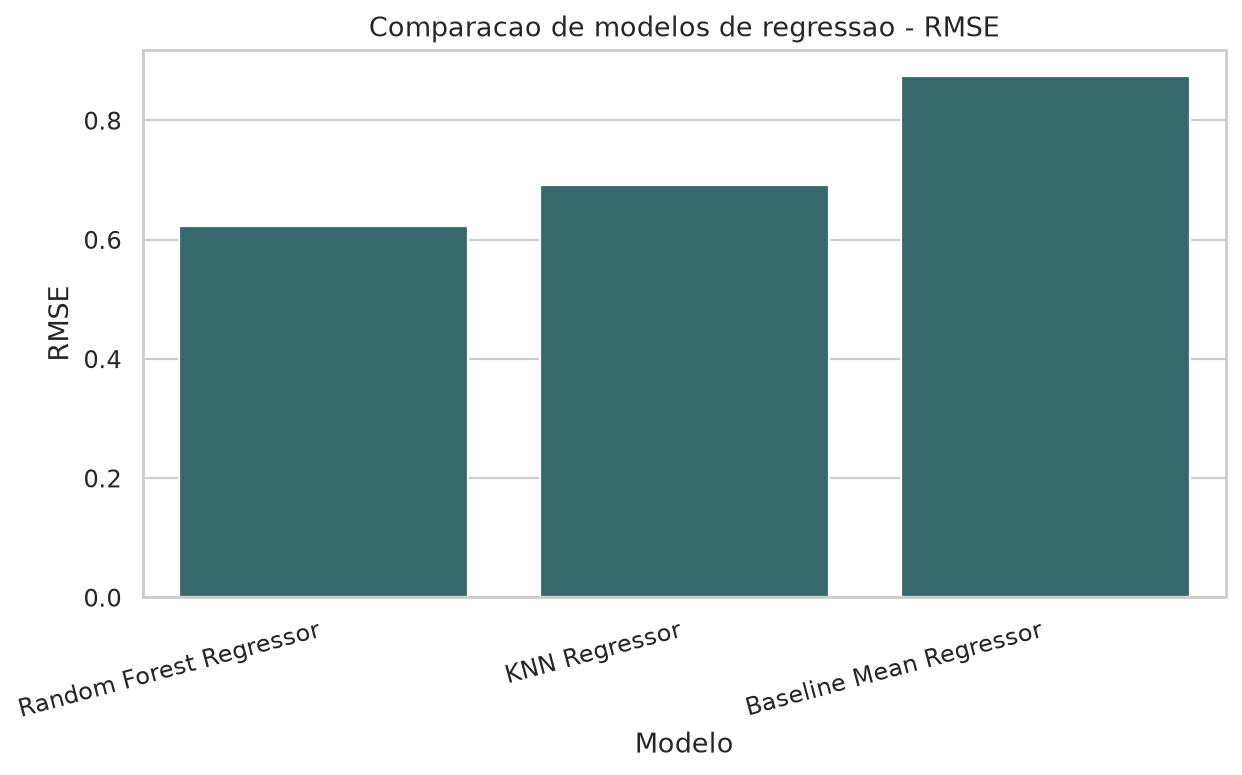
\includegraphics[width=\linewidth]{model_comparison_regression_rmse.png}
\end{minipage}
\hfill
\begin{minipage}{0.52\textwidth}
\centering
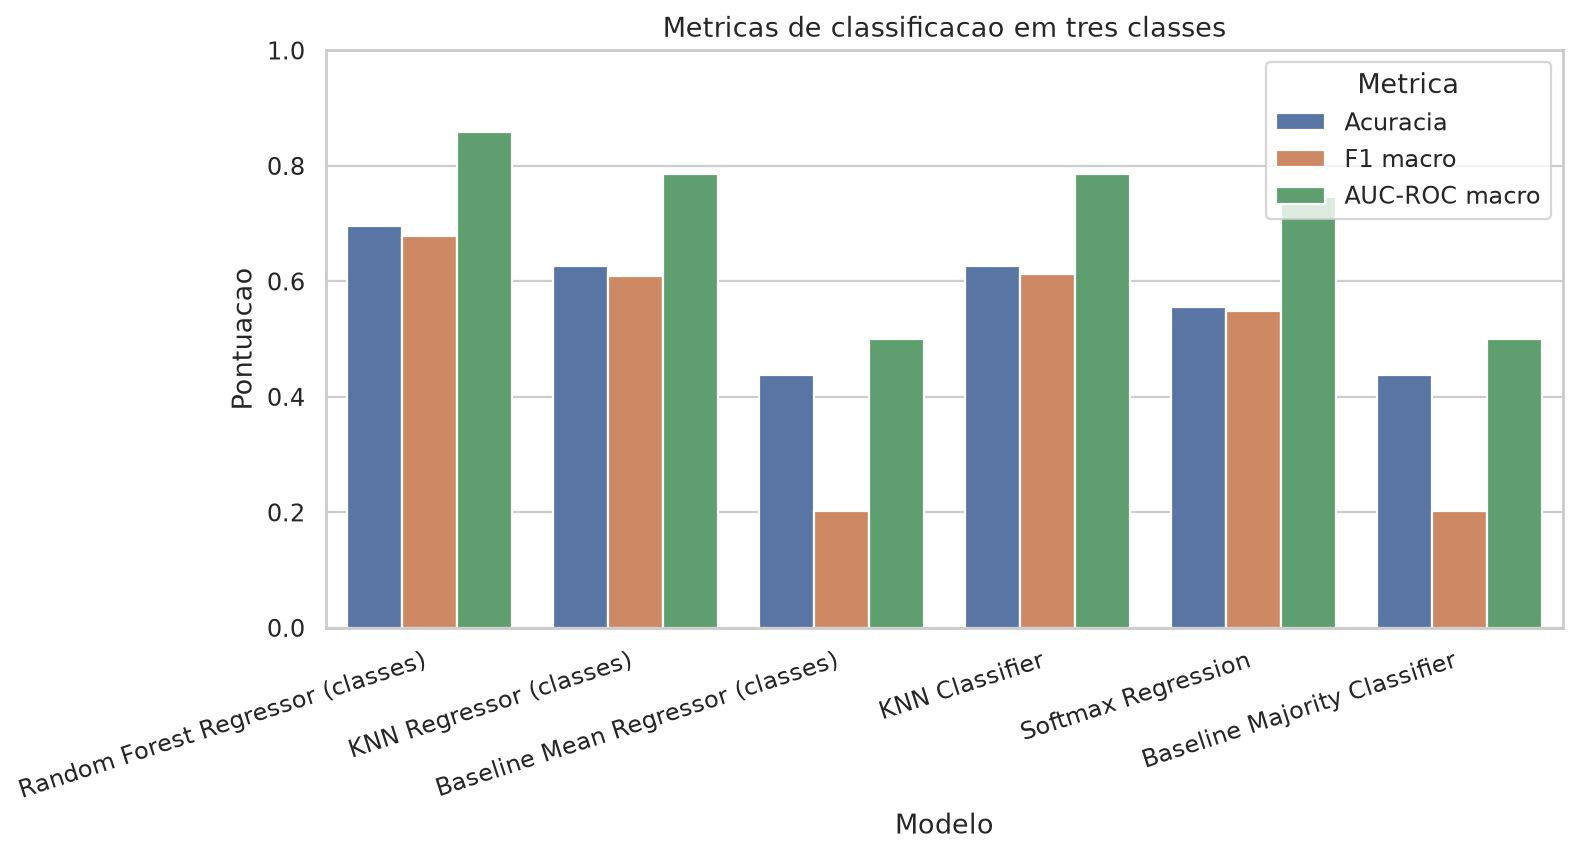
\includegraphics[width=\linewidth]{model_comparison_classification_metrics.png}
\end{minipage}
\caption{Compara\c{c}\~ao de desempenho em regress\~ao e em m\'etricas orientadas a classifica\c{c}\~ao, incluindo baselines triviais.}
\label{fig:comparacao-modelos}
\end{figure}

\subsection{Desempenho por classe}
\label{subsec:por-classe}

A Tabela~\ref{tab:por-classe} mostra que a avalia\c{c}\~ao por classe altera a interpreta\c{c}\~ao dos resultados agregados. A Random Forest convertida foi a melhor em desempenho geral, mas sua revoca\c{c}\~ao para a classe boa foi 0,4844, inferior \`a revoca\c{c}\~ao das classes ruim e mediana. Esse comportamento \'e compat\'ivel com o fato de a Random Forest ter sido treinada como regressora da nota cont\'inua, sem pondera\c{c}\~ao por classe: como a distribui\c{c}\~ao concentra muitos exemplos nas notas 5 e 6, a m\'edia das \'arvores tende a ser puxada para a regi\~ao central da escala. O KNN Classifier, embora inferior em acur\'acia e AUC-ROC macro, apresentou revoca\c{c}\~ao mais equilibrada entre as tr\^es classes. A Softmax Regression teve revoca\c{c}\~ao alta para vinhos bons, favorecida pela pondera\c{c}\~ao inversa \`a frequ\^encia das classes, mas revoca\c{c}\~ao baixa para vinhos medianos, o que explica sua menor acur\'acia.

\begin{table}[htbp]
\centering
\caption{Precis\~ao e revoca\c{c}\~ao por classe no conjunto de teste.}
\label{tab:por-classe}
\resizebox{\textwidth}{!}{%
\begin{tabular}{lrrrrrr}
\toprule
Modelo & Prec. ruim & Rev. ruim & Prec. mediano & Rev. mediano & Prec. bom & Rev. bom \\
\midrule
Random Forest Regressor & 0,7980 & 0,6625 & 0,6162 & 0,8169 & 0,8158 & 0,4844 \\
KNN Regressor & 0,7409 & 0,5996 & 0,5675 & 0,7183 & 0,6122 & 0,4688 \\
KNN Classifier & 0,6918 & 0,6918 & 0,5966 & 0,6250 & 0,5677 & 0,5078 \\
Softmax Regression & 0,6501 & 0,7128 & 0,5776 & 0,3539 & 0,4209 & 0,7070 \\
\bottomrule
\end{tabular}%
}
\end{table}

\begin{figure}[htbp]
\centering
\begin{minipage}{0.48\textwidth}
\centering
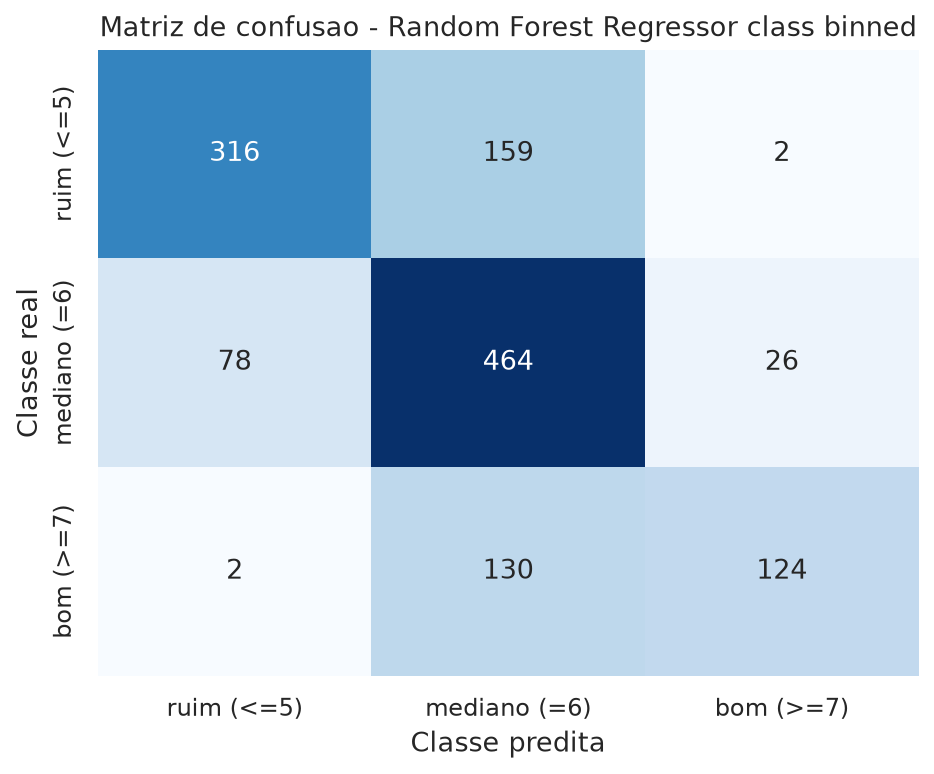
\includegraphics[width=\linewidth]{confusion_matrix_random_forest_regressor_class_binned.png}
\end{minipage}
\hfill
\begin{minipage}{0.48\textwidth}
\centering
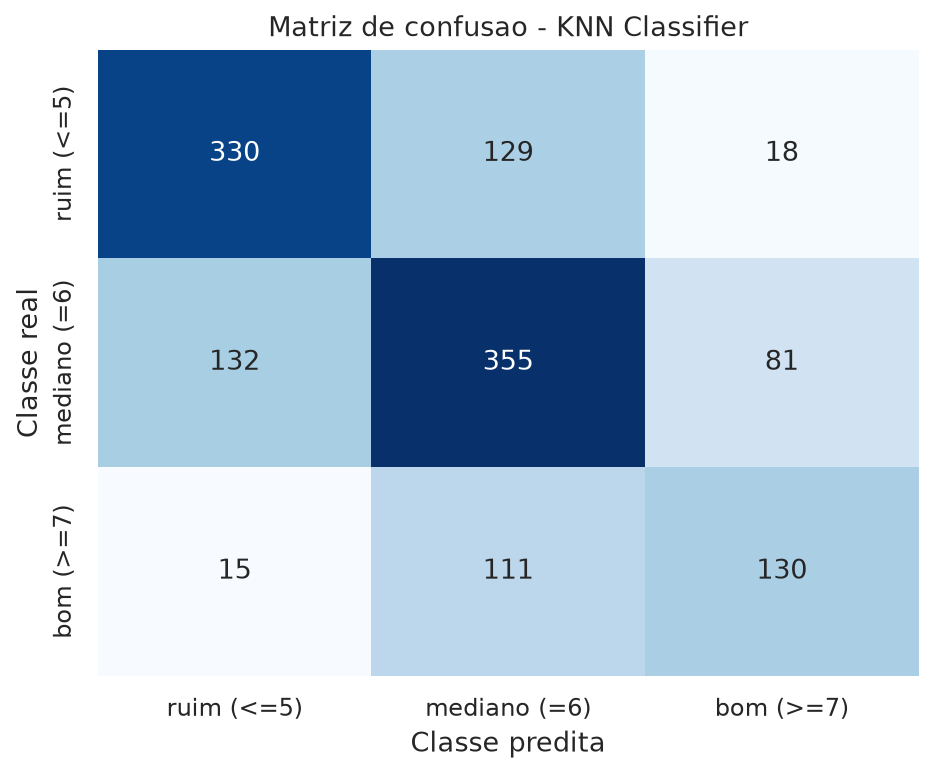
\includegraphics[width=\linewidth]{confusion_matrix_knn_classifier.png}
\end{minipage}
\caption{Matrizes de confus\~ao da Random Forest convertida para classes e do KNN Classifier.}
\label{fig:matrizes-confusao}
\end{figure}

As matrizes de confus\~ao da Figura~\ref{fig:matrizes-confusao} mostram que a maior parte dos erros ocorre entre classes adjacentes. Esse padr\~ao \'e coerente com a natureza ordinal do alvo: um vinho com nota 6 e outro com nota 7 podem ter perfis f\'isico-qu\'imicos pr\'oximos, embora sejam separados pela regra de agrupamento.

\subsection{Interpreta\c{c}\~ao dos modelos}
\label{subsec:interpretacao}

A Figura~\ref{fig:interpretacao} apresenta duas an\'alises complementares. Na Random Forest, a import\^ancia por redu\c{c}\~ao de impureza indicou maior contribui\c{c}\~ao relativa de densidade, teor alco\'olico e acidez vol\'atil. Essa interpreta\c{c}\~ao deve ser lida como descritiva, pois import\^ancias baseadas em impureza podem ser influenciadas por correla\c{c}\~oes entre atributos. A mesma cautela vale para a Regress\~ao Softmax: os coeficientes padronizados n\~ao devem ser interpretados como efeitos causais ou independentes, j\'a que atributos como densidade, teor alco\'olico e a\c{c}\'ucar residual s\~ao correlacionados. Ainda assim, como leitura associativa, os coeficientes indicaram padr\~oes coerentes: maior teor alco\'olico deslocou a decis\~ao em dire\c{c}\~ao \`a classe boa e contra a classe ruim, enquanto maior acidez vol\'atil deslocou a decis\~ao no sentido oposto.

\begin{figure}[htbp]
\centering
\begin{minipage}{0.48\textwidth}
\centering
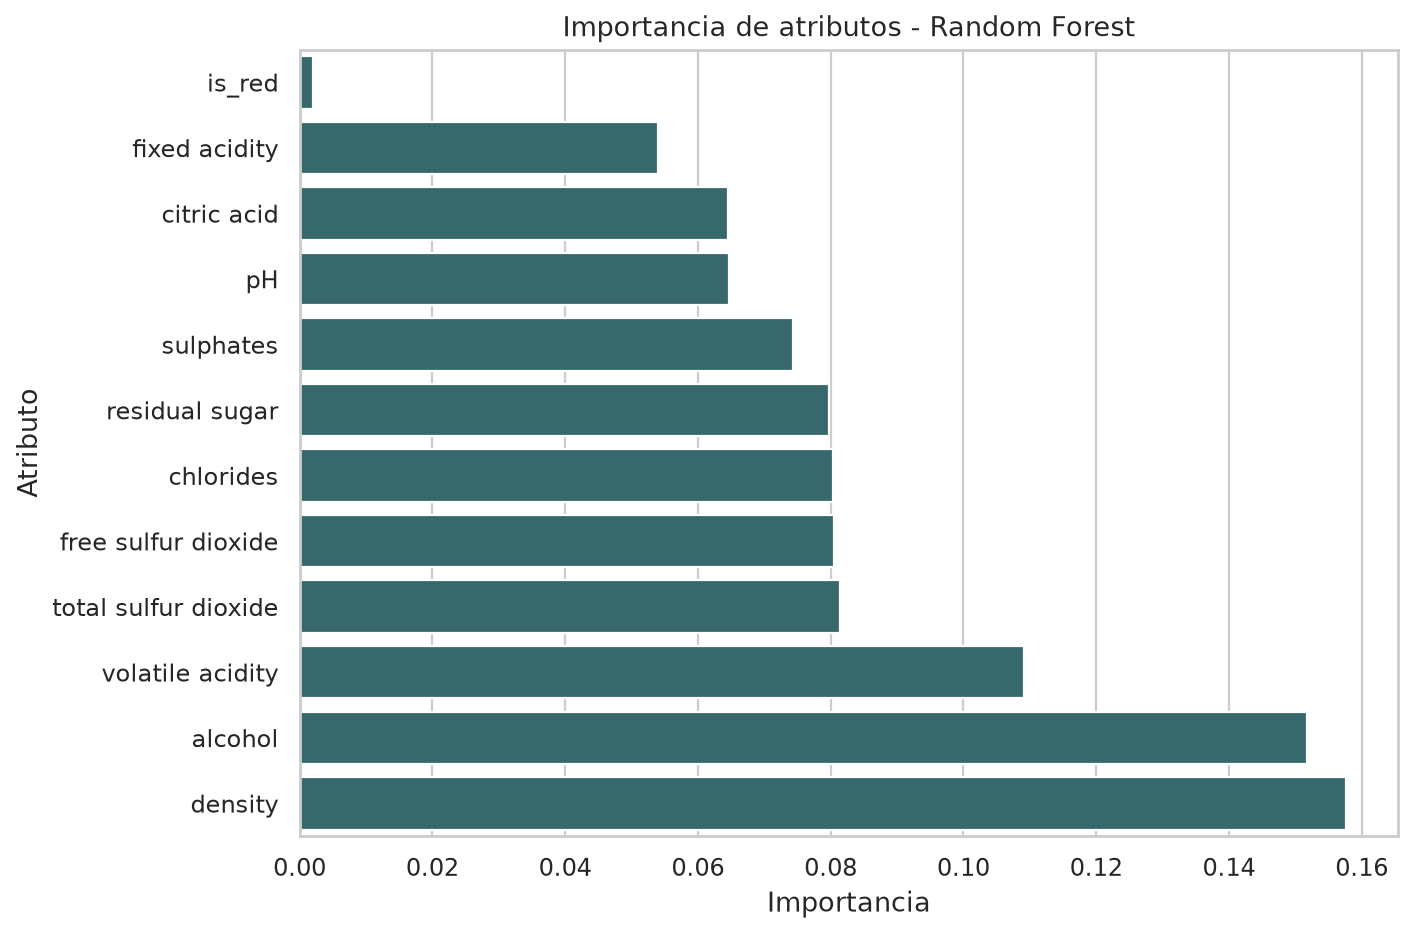
\includegraphics[width=\linewidth]{rf_feature_importance_regressor.png}
\end{minipage}
\hfill
\begin{minipage}{0.48\textwidth}
\centering
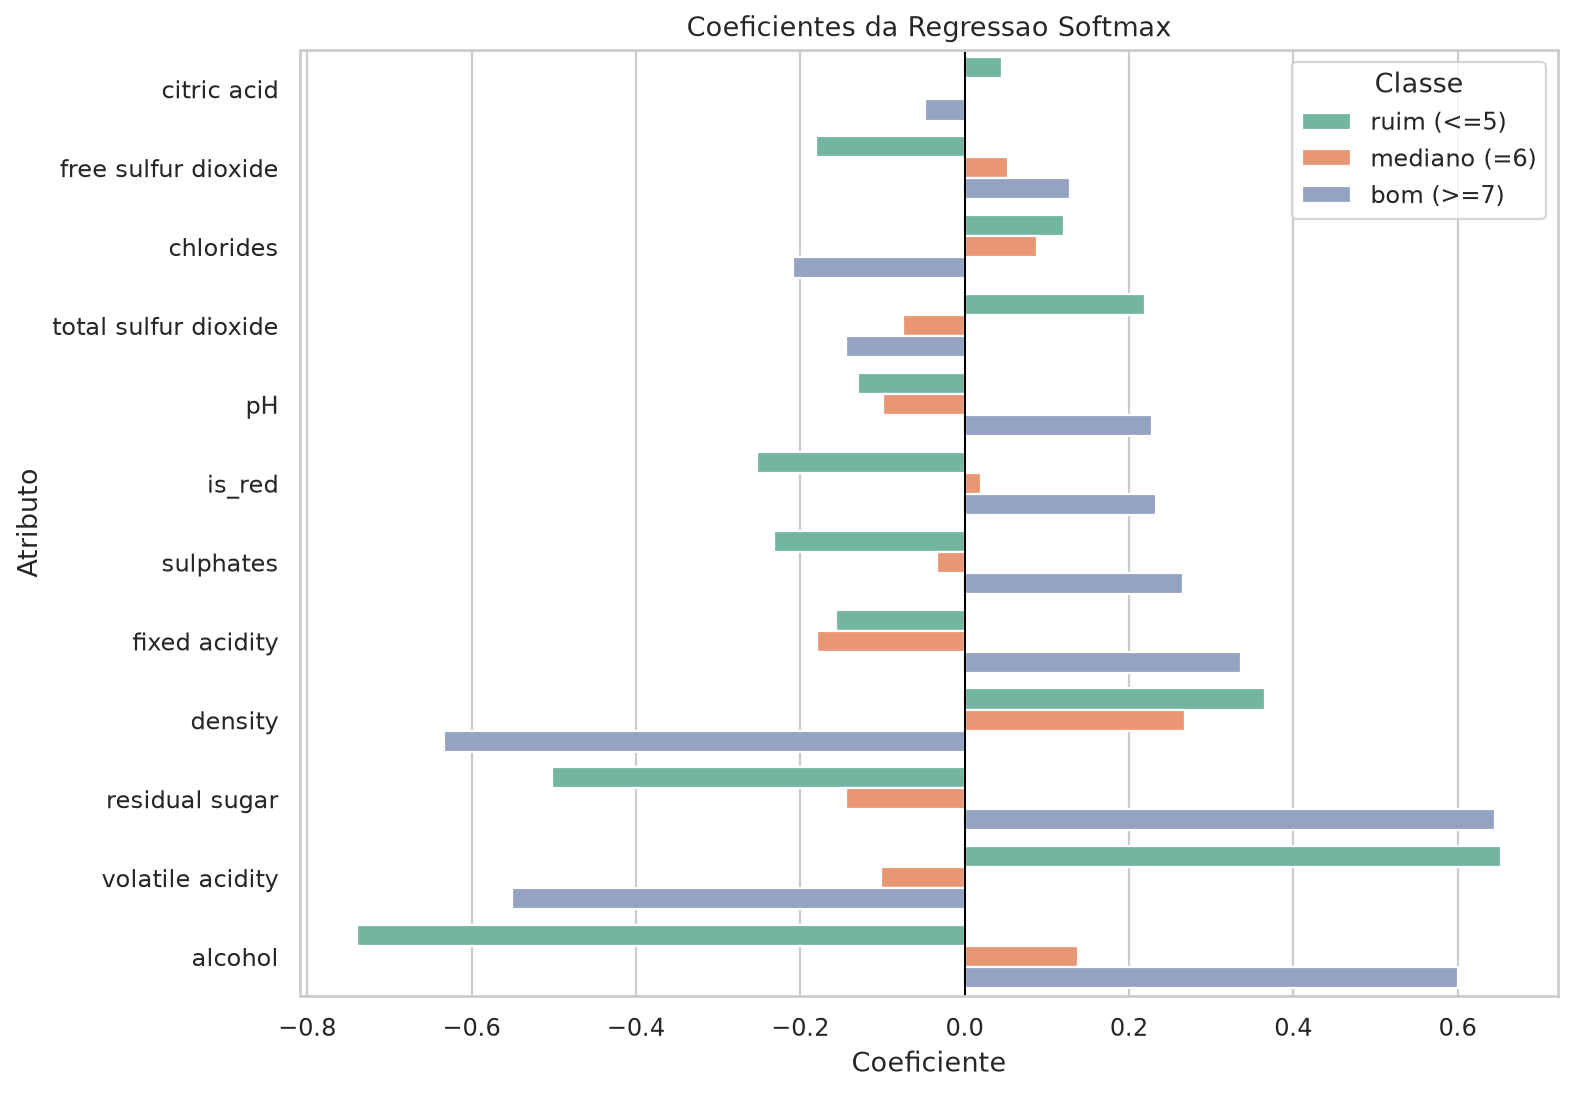
\includegraphics[width=\linewidth]{softmax_coefficients.png}
\end{minipage}
\caption{Import\^ancia de atributos da Random Forest e coeficientes padronizados da Regress\~ao Softmax.}
\label{fig:interpretacao}
\end{figure}

Em conjunto, os resultados indicam que a predi\c{c}\~ao de qualidade baseada apenas em medi\c{c}\~oes f\'isico-qu\'imicas \'e poss\'ivel, mas limitada. O melhor $R^2$ foi 0,4917, ou seja, cerca de metade da variabilidade da nota permaneceu n\~ao explicada pelo melhor modelo avaliado. Isso \'e plaus\'ivel, pois a base n\~ao inclui informa\c{c}\~oes como safra, produtor, variedade da uva, pre\c{c}o, condi\c{c}\~oes de armazenamento ou descritores sensoriais detalhados.

\section{Limita\c{c}\~oes e Amea\c{c}as \`a Validade}
\label{sec:limitacoes}

A primeira limita\c{c}\~ao \'e que a avalia\c{c}\~ao repetida usou apenas cinco particionamentos e manteve fixos os hiperpar\^ametros selecionados na execu\c{c}\~ao principal. Assim, os intervalos de confian\c{c}a descrevem a varia\c{c}\~ao dos modelos finais sob diferentes divis\~oes treino--teste, mas n\~ao incluem a variabilidade que surgiria se toda a sele\c{c}\~ao de hiperpar\^ametros fosse repetida em cada particionamento.

A segunda limita\c{c}\~ao \'e a defini\c{c}\~ao das classes. Agrupar notas em ruim, mediano e bom melhora a interpreta\c{c}\~ao, mas reduz a granularidade da escala original e cria fronteiras r\'igidas entre notas vizinhas. Al\'em disso, os classificadores diretos n\~ao foram modelos ordinais; eles tratam as classes como categorias nominais, apesar de haver ordem natural.

A terceira limita\c{c}\~ao est\'a no espa\c{c}o de modelos e hiperpar\^ametros. Por restri\c{c}\~ao de implementa\c{c}\~ao manual e custo computacional, a busca foi deliberadamente pequena, inclusive para a Random Forest. Modelos adicionais, como gradient boosting, SVMs, redes neurais e regress\~ao ordinal, poderiam alterar o ranqueamento de desempenho.

A quarta limita\c{c}\~ao \'e que o tratamento do desbalanceamento n\~ao foi sim\'etrico entre os modelos. A Regress\~ao Softmax usou pesos inversamente proporcionais \`as frequ\^encias de classe, enquanto Random Forest e KNN Regressor foram treinados sobre a nota cont\'inua sem pondera\c{c}\~ao espec\'ifica para as classes derivadas. Assim, parte da diferen\c{c}a entre modelos reflete tamb\'em a formula\c{c}\~ao adotada, n\~ao apenas a fam\'ilia algor\'itmica.

A quinta limita\c{c}\~ao decorre das implementa\c{c}\~oes manuais. Embora as m\'etricas, parti\c{c}\~oes e resultados sejam reprodut\'iveis pelo script, n\~ao foi executado neste trabalho um teste de equival\^encia em dados de brinquedo contra implementa\c{c}\~oes consolidadas, como as do \textit{scikit-learn}. Esse tipo de sanity check reduziria o risco de erro de implementa\c{c}\~ao.

A sexta limita\c{c}\~ao \'e a presen\c{c}a de linhas duplicadas na base original. As duplicatas foram verificadas e relatadas antes da divis\~ao treino--teste, mas n\~ao foram removidas para manter comparabilidade direta com os arquivos originais. Remover ou agrupar duplicatas poderia alterar as estimativas finais.

Por fim, a validade externa \'e limitada pela pr\'opria base. As amostras pertencem a vinhos Vinho Verde e cont\^em apenas medi\c{c}\~oes f\'isico-qu\'imicas. Assim, os resultados n\~ao devem ser generalizados automaticamente para outros estilos de vinho, regi\~oes ou processos de avalia\c{c}\~ao sensorial.

\section{Conclus\~ao}
\label{sec:conclusao}

Este trabalho avaliou a predi\c{c}\~ao da qualidade de vinhos a partir de atributos f\'isico-qu\'imicos usando modelos implementados manualmente. A compara\c{c}\~ao incluiu regress\~ao da nota original e classifica\c{c}\~ao em tr\^es faixas ordinais. O protocolo experimental buscou reduzir vazamento de informa\c{c}\~ao, preservar a distribui\c{c}\~ao das classes e reportar m\'etricas adequadas ao desbalanceamento.

A Random Forest Regressor foi o modelo com melhor desempenho geral no teste, com RMSE de 0,6235, $R^2$ de 0,4917 e AUC-ROC macro de 0,8582 ap\'os convers\~ao das predi\c{c}\~oes para classes, superando claramente os baselines triviais. Em cinco divis\~oes repetidas, o RMSE m\'edio foi 0,6225 $\pm$ 0,0023. Entre os classificadores diretos, o KNN Classifier superou a Regress\~ao Softmax nas m\'etricas agregadas. Esses resultados favorecem modelos n\~ao lineares para o problema, mas tamb\'em mostram que a classe de vinhos bons permanece dif\'icil de recuperar com alta revoca\c{c}\~ao e que a Random Forest apresenta hiato relevante entre treino e teste.

Como trabalhos futuros, recomenda-se avaliar modelos ordinais, repetir tamb\'em a sele\c{c}\~ao de hiperpar\^ametros dentro de uma valida\c{c}\~ao cruzada externa, testar estrat\'egias de calibra\c{c}\~ao e repondera\c{c}\~ao para a classe boa, estudar o efeito de remover duplicatas, e comparar as implementa\c{c}\~oes manuais com bibliotecas consolidadas em dados de brinquedo. Essas extens\~oes permitiriam separar limita\c{c}\~oes do conjunto de dados, limita\c{c}\~oes dos algoritmos e limita\c{c}\~oes da implementa\c{c}\~ao.

\section*{Contribui\c{c}\~ao dos Participantes}

Todos os integrantes contribu\'iram para as diferentes etapas do projeto, incluindo a escrita e revis\~ao do artigo, a programa\c{c}\~ao, a implementa\c{c}\~ao dos modelos e a execu\c{c}\~ao dos experimentos. Gabriel de Sousa Cavalcante e Maria Elaine de Holanda Cavalcante tiveram maior foco na elabora\c{c}\~ao do artigo, tamb\'em participando da programa\c{c}\~ao. Gabriel Matias de Almeida e Edileudo Maciel Moreira Filho tiveram maior foco na programa\c{c}\~ao e implementa\c{c}\~ao dos modelos, tamb\'em participando da revis\~ao do artigo.

\begin{thebibliography}{99}

\bibitem{cortez2009modeling}
P. Cortez, A. Cerdeira, F. Almeida, T. Matos e J. Reis.
\newblock Modeling wine preferences by data mining from physicochemical properties.
\newblock \textit{Decision Support Systems}, 47(4):547--553, 2009.
\newblock \url{https://doi.org/10.1016/j.dss.2009.05.016}.

\bibitem{uciWineQuality}
P. Cortez, A. Cerdeira, F. Almeida, T. Matos e J. Reis.
\newblock Wine Quality [Dataset].
\newblock UCI Machine Learning Repository, 2009.
\newblock \url{https://doi.org/10.24432/C56S3T}.

\bibitem{breiman2001random}
L. Breiman.
\newblock Random Forests.
\newblock \textit{Machine Learning}, 45:5--32, 2001.
\newblock \url{https://doi.org/10.1023/A:1010933404324}.

\bibitem{breiman1984cart}
L. Breiman, J. H. Friedman, R. A. Olshen e C. J. Stone.
\newblock \textit{Classification and Regression Trees}.
\newblock Wadsworth, 1984.

\bibitem{cover1967nearest}
T. M. Cover e P. E. Hart.
\newblock Nearest neighbor pattern classification.
\newblock \textit{IEEE Transactions on Information Theory}, 13(1):21--27, 1967.
\newblock \url{https://doi.org/10.1109/TIT.1967.1053964}.

\bibitem{bishop2006pattern}
C. M. Bishop.
\newblock \textit{Pattern Recognition and Machine Learning}.
\newblock Springer, 2006.

\bibitem{fawcett2006roc}
T. Fawcett.
\newblock An introduction to ROC analysis.
\newblock \textit{Pattern Recognition Letters}, 27(8):861--874, 2006.
\newblock \url{https://doi.org/10.1016/j.patrec.2005.10.010}.

\bibitem{hand2001auc}
D. J. Hand e R. J. Till.
\newblock A simple generalisation of the area under the ROC curve for multiple class classification problems.
\newblock \textit{Machine Learning}, 45:171--186, 2001.
\newblock \url{https://doi.org/10.1023/A:1010920819831}.

\end{thebibliography}

\end{document}
